\mode*

\section[Hash functions]{What was a hash function now again?}

\begin{frame}
  \begin{definition}[One-way function\footfullcite{GoldreichFOC-1}]
    \begin{itemize}
      \item Let \(h\colon \{0,1\}^*\to \{0,1\}^*\).
      \item \(h\) is \emph{one-way} if
        \begin{enumerate}
          \item there exists an efficient algorithm \(A\) such that \(A(x) 
              = h(x)\);
          \item for every efficient algorithm \(A^\prime\), every positive 
            polynomial \(p(\cdot)\) and all sufficiently large \(n\)'s
            \[\Prob{A^\prime(h(x), 1^n) \in h^{-1}(h(x))} < \frac{1}{p(n)}\]
        \end{enumerate}
    \end{itemize}
  \end{definition}
\end{frame}

\begin{frame}
  \begin{definition}[Preimage resistance (one way)]
    \begin{description}
      \item[Input] hash function~\(H\), value~\(y\).
      \item[Output] Any \(x\) such that \(H(x) = y\).
    \end{description}
  \end{definition}

  \begin{definition}[Second preimage resistance (weak collision resistance)]
    \begin{description}
      \item[Input] hash function~\(H\), value \(x\).
      \item[Output] Any value \(x'\) such that \(H(x) = H(x')\).
    \end{description}
  \end{definition}

  \begin{definition}[Collision resistance (strong collision resistance)]
    \begin{description}
      \item[Input] hash function~\(H\).
      \item[Output] Any two \(x, x'\) such that \(H(x) = H(x')\).
    \end{description}
  \end{definition}
\end{frame}


\section[Chaining]{Chaining and block chains}


\section{Proof-of-work}


\section{Tree hashing}

\begin{frame}
  \begin{figure}
    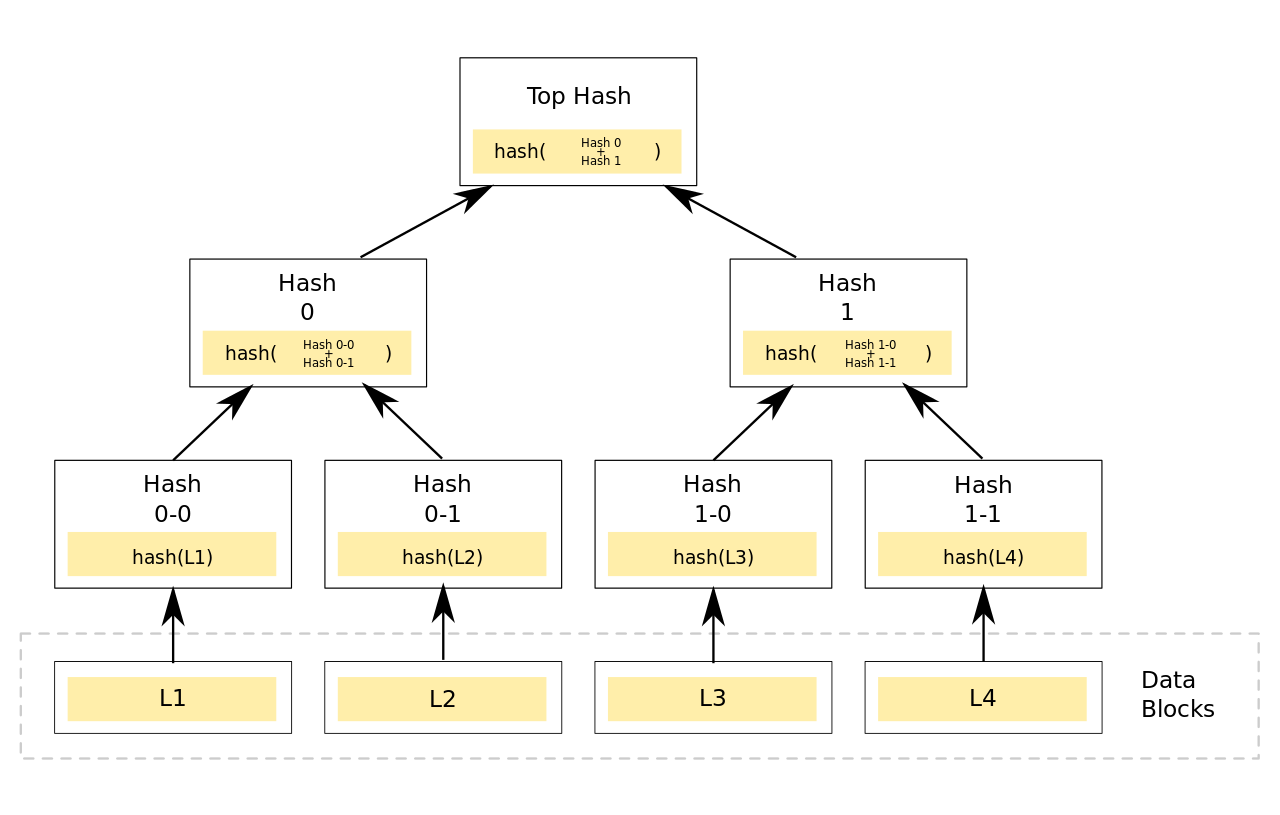
\includegraphics[width=0.9\columnwidth]{fig/merkle-tree.png}
    \caption{Merkle tree}
  \end{figure}
\end{frame}

\subsection{Transactions on blockchains}

\begin{frame}
  \begin{example}[Transactions]
    \begin{itemize}
      \item Transaction~\(T_i\) is in block \(B_j\).
      \item Compute \(h = H(T_i)\).
      \item Check if \(h\) is among the leaves in the Merkle tree of 
        transactions in \(B_j\).
    \end{itemize}
  \end{example}
\end{frame}

